\begin{center}
\begin{minipage}[h]{0.9\linewidth}
\begin{wrapfigure}{l}{0.42\textwidth}
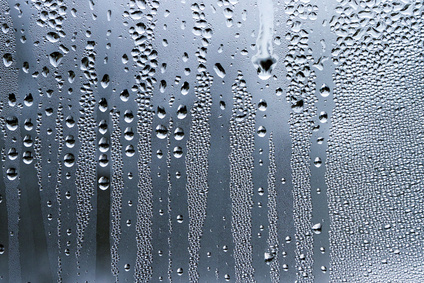
\includegraphics[width=0.42\textwidth]{graphics/luftfeuchtigkeit.jpg}
\\
\end{wrapfigure}
	
\NewsItem{Grundlagen der Luftfeuchtigkeitsmessung}
\vspace{3pt}

%%======================================================================== Text Einfügen
Wichtig für das allgemeine Verständnis der Feuchtemessung ist, dass es unterschiedliche Verfahren zur Messung der Feuchte gibt. Dabei befassen sich diese mit gasförmigen (z.B. Luft), flüssigen oder festen Stoffen. Die feuchte Luft ist demnach eine Mischung von trockener Luft und Wasserdampf, dessen Sättigungspunkt abhängig des Barometerstands und der Umgebungstemperatur ist.

\end{minipage}
\end{center}